% This is "sig-alternate.tex" V2.1 April 2013
% This file should be compiled with V2.5 of "sig-alternate.cls" May 2012
%
% This example file demonstrates the use of the 'sig-alternate.cls'
% V2.5 LaTeX2e document class file. It is for those submitting
% articles to ACM Conference Proceedings WHO DO NOT WISH TO
% STRICTLY ADHERE TO THE SIGS (PUBS-BOARD-ENDORSED) STYLE.
% The 'sig-alternate.cls' file will produce a similar-looking,
% albeit, 'tighter' paper resulting in, invariably, fewer pages.
%
% ----------------------------------------------------------------------------------------------------------------
% This .tex file (and associated .cls V2.5) produces:
%       1) The Permission Statement
%       2) The Conference (location) Info information
%       3) The Copyright Line with ACM data
%       4) NO page numbers
%
% as against the acm_proc_article-sp.cls file which
% DOES NOT produce 1) thru' 3) above.
%
% Using 'sig-alternate.cls' you have control, however, from within
% the source .tex file, over both the CopyrightYear
% (defaulted to 200X) and the ACM Copyright Data
% (defaulted to X-XXXXX-XX-X/XX/XX).
% e.g.
% \CopyrightYear{2007} will cause 2007 to appear in the copyright line.
% \crdata{0-12345-67-8/90/12} will cause 0-12345-67-8/90/12 to appear in the copyright line.
%
% ---------------------------------------------------------------------------------------------------------------
% This .tex source is an example which *does* use
% the .bib file (from which the .bbl file % is produced).
% REMEMBER HOWEVER: After having produced the .bbl file,
% and prior to final submission, you *NEED* to 'insert'
% your .bbl file into your source .tex file so as to provide
% ONE 'self-contained' source file.
%
% ================= IF YOU HAVE QUESTIONS =======================
% Questions regarding the SIGS styles, SIGS policies and
% procedures, Conferences etc. should be sent to
% Adrienne Griscti (griscti@acm.org)
%
% Technical questions _only_ to
% Gerald Murray (murray@hq.acm.org)
% ===============================================================
%
% For tracking purposes - this is V2.0 - May 2012

\documentclass{sig-alternate-05-2015}

\usepackage{mathtools}
\usepackage{algorithm}
\usepackage{algpseudocode}
\begin{document}

% Copyright
%\setcopyright{acmcopyright}
%\setcopyright{acmlicensed}
%\setcopyright{rightsretained}
%\setcopyright{usgov}
%\setcopyright{usgovmixed}
%\setcopyright{cagov}
%\setcopyright{cagovmixed}


%\CopyrightYear{2007} % Allows default copyright year (20XX) to be over-ridden - IF NEED BE.
%\crdata{0-12345-67-8/90/01}  % Allows default copyright data (0-89791-88-6/97/05) to be over-ridden - IF NEED BE.
% --- End of Author Metadata ---

\title {Analysis of the common reccommendation systems with the common frameworks: Spark and Flink}
\subtitle{ Final Report for the BigData project}
%
% You need the command \numberofauthors to handle the 'placement
% and alignment' of the authors beneath the title.
%
% For aesthetic reasons, we recommend 'three authors at a time'
% i.e. three 'name/affiliation blocks' be placed beneath the title.
%
% NOTE: You are NOT restricted in how many 'rows' of
% "name/affiliations" may appear. We just ask that you restrict
% the number of 'columns' to three.
%
% Because of the available 'opening page real-estate'
% we ask you to refrain from putting more than six authors
% (two rows with three columns) beneath the article title.
% More than six makes the first-page appear very cluttered indeed.
%
% Use the \alignauthor commands to handle the names
% and affiliations for an 'aesthetic maximum' of six authors.
% Add names, affiliations, addresses for
% the seventh etc. author(s) as the argument for the
% \additionalauthors command.
% These 'additional authors' will be output/set for you
% without further effort on your part as the last section in
% the body of your article BEFORE References or any Appendices.

\numberofauthors{2} %  in this sample file, there are a *total*
% of EIGHT authors. SIX appear on the 'first-page' (for formatting
% reasons) and the remaining two appear in the \additionalauthors section.
%
\author{
% You can go ahead and credit any number of authors here,
% e.g. one 'row of three' or two rows (consisting of one row of three
% and a second row of one, two or three).
%
% The command \alignauthor (no curly braces needed) should
% precede each author name, affiliation/snail-mail address and
% e-mail address. Additionally, tag each line of
% affiliation/address with \affaddr, and tag the
% e-mail address with \email.
%
% 1st. author
\alignauthor
Mirko Morandi\\
       \affaddr {University of Trento}\\
       \affaddr {176043}\\
       \email {mirko.morandi@unitn.it}\\
% 2nd. author
\alignauthor
Zhiheng Xu\\
        \affaddr {University of Trento}\\
        \affaddr {174222}\\
        \email {zhiheng.xu@unin.it}\\
}

% Just remember to make sure that the TOTAL number of authors
% is the number that will appear on the first page PLUS the
% number that will appear in the \additionalauthors section.

\maketitle
\begin{abstract}

In this paper we provide an extensive analysis of the actual state of the
art of recommendation systems.\\
\textit{Collaborative Filtering} is the current buzzword in the
world of recommendations, came to notoriety after the Netflix Prize
challenge. In this paper we aim to analyze the current implementations
of two different algorithms used for Collaborative Filtering: \textbf{Alternating Least Squares} (ALS) and \textbf{Stochastic
Gradient Descent} (SGD) in combination with the common frameworks \texttt{Spark}.
\end{abstract}




\keywords{Spark; CF; Collaborative Filtering; ALS; SGD; Scala}

\section{Introduction}
Recommender systems are now trending due to the overwhelming availability
of data. These systems have the ability to discover hidden relationships between
users and items, and use these patterns to improve the user's taste prediction.
Researchers discovered a "neighbourhood" of users with a similar taste
which can be revealed by their previous actions: both implicit and explicit.
\texttt{Collaborative filtering} is by far the most common approach adapted also by
some of the biggest companies in the IT sector such as: \textbf{Amazon}, \textbf{Facebook} and \textbf{Netflix}.
Although it's massive presence in the market, \texttt{CF} is not the only approach
available for a recommendation system, but it is actually the successor of
\texttt{Content-Based filtering}. The latter aims to profile a user searching
the correlation with the item's peculiarity. By item peculiarity we refer to
its implicit and explicit characteristics, for example a song's genre,
subgenre, writer, composer, year of composition, beats per second etc.
The problem with this approach lays in the difficult of retrieving all the necessary
information, which sometimes are not even available or discloable.
Furthermore with the raise of the Big Data paradigm some frameworks started to grow from
the academic world to the Apache Foundation: \textbf{Flink} and \textbf{Spark}.
Those frameworks can be seen an extension of the Hadoop ecosystem, and both of them
have their own pros and cons which will be briefly analyzed further in this paper.






\section{Collaborative Filtering}

The paper is structured as follow: description in more details
of \texttt{Collaborative Filtering} with it's problems, what are
the most common algorithms used with \texttt{CF} and a brief
introduction to both \textbf{Flink} and \textbf{Spark}.



\subsection{Collaborative Filtering Approaches}


Collaborative Filtering can be subsenquently defined in two
different approaches:

\subsubsection{Memory-based Collaborative Filtering}
In \texttt{memory-based CF} uses user ratings to compute similarity
between user and items and subsequently make a recommendation. Usually
this approach involves "neighboring" algorithms such as \textbf{K-Nearest Neighbours}
to build relationships between users. The similarity between two users
is calculated using the \textbf{cosine similarity}.\\
\textbf{Cosine similarity} is a measure of similarity between two vectors of an inner product space that measures the cosine of the angle between them.[4]
\begin{equation}
\cos ({\bf t},{\bf e})= {{\bf t} {\bf e} \over \|{\bf t}\| \|{\bf e}\|} = \frac{ \sum_{i=1}^{n}{{\bf t}_i{\bf e}_i} }{ \sqrt{\sum_{i=1}^{n}{({\bf t}_i)^2}} \sqrt{\sum_{i=1}^{n}{({\bf e}_i)^2}} }
\end{equation}
The recommendation is made by finding the top K similar users and aggregate their
user-item matrices to find the appropriate recommendation.
The typical problem of this approach is the difficult with scaling
when the data gets bigger. Due to the \texttt{Big Data} paradigm expansion
this approach has been deprecated favoring the following approach.


\subsubsection{Model-based Collaborative Filtering}
The most common approach to \texttt{CF} is through the factorization
of a very big and sparse matrix.[3] For example during the Netflix
Prize at the participants were given a matrix of 8.5 billions of ratings,
of which only 100 millions were non zero values.
\textit{Model-based CF} uses machine-learning and data mining algorithms
to uncover the latent factor model between users and items to
predict the missing ratings.\textbf{latent factor models} are hidden
relationships between users and items hardly discoverable in the original data;
usually they may for example denote the quantity of action in a movie or the complexity
of the characters.These vectors are then used to create the missing values in the user-items
matrix.\\


Furthermore the model-based content filtering can be expanded in two distinct sections:
\textit{user and item based content filtering} depending on the priority given to the
prediction.


\subsection{Related problems}
\subsubsection{Cold start problem}
Due to the nature of CF, the system needs a huge amount of data
in order to produce a reliable prediction. But what happens if our system
hasn't collected any or not enough information yet?
This problem is called \textbf{cold start} and can be tackled with some advanced
machine learning solutions called \textit{active learning}.

\subsubsection{Shilling Attacks}
CF can be exploited to perturbate its prediction system with a technique
called \textit{shilling attacks}. This happens when the input system (e.g. ratings)
are given in the correct way trying to alter the recommendations to the one
favoured by the attacker. It has also been noticed that these kind of attacks affect
more user-based CF algorithms instead of item-based.[5]

\subsubsection{Sparsity}

In the era of the \textit{web 2.0} the matrices who compose the datasets are
usually very sparse due to the typical proportion for which  \(nUsers \ll nItems\).
As said previously the matrix which was given had only 100M ratings out of
8.5 billions of records. This problem is solved using matrix factorization.

%[TODO] correct all the formulas
\section{Matrix Factorization}

During the last decade a huge effort has been applied to solve the problem of
big datasets with an incredible amount of data.
Let denote $R = r_{ij}$ denote a
user-movie where each element $r_{ij}$ represents a rating given by
a user \textit{i} to an item \textit{j} with a value from 0 to 5; where 0 means
non rated and 1 to 5 a rating ranging relatively from \textit{very poor} to \textit{awesome}.
Let also define \textit{m} the number of users and \textit{n} the number of movies in the system.
The problem of \textit{recommender systems} is to predict the missing values of $R$
using the known ratings.\\
\begin{table}
\centering
\caption{Example of a sparse user-item ratings matrix}
\begin{tabular}{|c|c|c|c|c|c|} \hline
items/users  & \textbf{U1} & \textbf{U2} & \textbf{U3} & \textbf{U4} & \textbf{U5}\\ \hline
\textbf{I1} & 5 & 3 & - & 1 &  3  \\ \hline
\textbf{I2} & 4 & - & 2 & 1 &  -  \\ \hline
\textbf{I3} & 2 & 2 & - & 5 &  - \\ \hline
\textbf{I4} & 4 & 3 & - & 4 &  2  \\ \hline
\textbf{I5} & - & 5 & 5 & 4 &  5  \\ \hline
\end{tabular}
\end{table}
The concept behind \textit{matrix factorization} is to find two matrices
$V,W$ relatively \textit{\textbf{m}} x \textit{\textbf{p}},\textit{\textbf{n}} x \textit{\textbf{p}}. which product
can approximate a much bigger matrix $R$ of dimensions \textit{\textbf{m}} x \textit{\textbf{n}}.\\
    %\textit{R} \(\approx\) \textit{V} * \textit{W}
    $R \approx V * W^T $
}\\
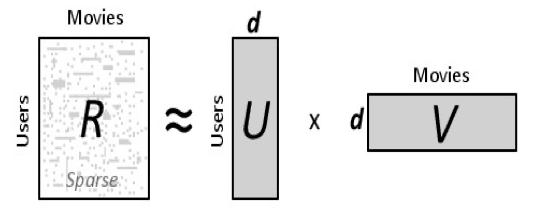
\includegraphics[scale=0.45]{matrix_factorization.png}
The process consists in a low-rank approximation of the user-item matrix using
for both users and items some feature vectors which are used to model
the prediction with a inner vector product of the selected user and item.\\
Ideally $r_{ij}$ should correspond to the predicted rating
but in reality the value will be different. Therefore we need a
loss function to determine the difference between \textbf{real value}
and \textbf{predicted value}. In our paper we are going to use the
\textbf{Root Mean Square Error},\\
\begin{equation}
{\sqrt {\frac{1} {N}{\sum\limits_{i,j}^N {(pr_{ij} - {r}_{ij} } })^{2} } }
\end{equation}
Where respectively \textit{prij} is the prediction for the rating
given by the user \textit{i} for an item \textit{j} and \textit{rij}
is the real rating for the former user and item.
The prediction is obtained with the dot product of the user-item vectors,(\textit{ui},\textit{vj})

\begin{equation}
    { prediction_{ij} = \bar{u}_{i} * \bar{v}_{j} }
\end{equation}
The low rank approximation problem is formulated as follows to
learn the factor vectors (u\textit{i},v\textit{j}) [6]

\begin{equation}
    {(u_{i},v_{j}) = \min_{u,v} {\sum\limits_{(u,i) \in K} {(pr_{u,v} - r_{u,v})}^{2} }}
\end{equation}

However solving the approximation with the former approach leads to the overfitting of data.
Overfitting means that our model is learning through the noise in the training data instead
of the underlying relations for which we expect to work. Although the performance will continue
improving with the training data it will get worse on unseen data. This usually happens
when we are using a too complex model or we have too many free parameters, and the latter is our case.
The solution is to apply regularization penzaling the magnitude of the feature vectors proportionally with a constant
factor \(\lambda\) obtaining the following and well known formula for low-rank approximation:\\


\begin{equation}
    {(u_{i},v_{j}) = \min_{u,v} {\sum\limits_{(u,i) \in K} {(pr_{u,v} - r_{u,v})}^{2} + \lambda(u_{i}^{2} + v_{j}^{2}) }}
\end{equation}


\subsection{Approaches}
There are mainly two approaches to minimize equation(5) and are known as:\\
\textbf{Alternating Least Square} and \textbf{Stochastic Gradient Descent}.

\subsection{Stochastic Gradient Descent}

\textit{Stochastic Gradient Descent} is a gradient descent optimization used
to minimize a loss function, in our case equation (5).
The goal of \textit{Stochastic Gradient Descent} is to find a value
$\theta^{*} \in R^{k} (k \geq 1) $ that minimizes a given loss $L(\theta)$.
The algorithm makes use of noisy observations $\bar{L}^{\prime}(\theta)$
of $L^{\prime}(\theta)$, the function's gradient with respect to $\theta$.
Starti with some initial value $\theta_{0}$, SGD refines the parameter
value by iterating the stochastic difference equation[7]

\begin{equation}
    {\theta_{n+1} = \theta_{n} - \epsilon_{n} \bar{L}^{\prime}(\theta_{n})}
\end{equation}

where $n$ denotes the step number and $\epsilon_{n}$ is a sequence of
decreasing step size.

\subsubsection{SGD with Matrix Factorization}

In matrix factorization we set $\theta = (V,W)$ and the loss function
can be written as $ Q(w) = {\sum Q(u,i)}$. Where $w$ is an approximation
obtained iterating through every single sample until a minimum is reached with
the following step: $w= w - aplha * d{\frac dw}(Q_{i}(w)) $
In our case $Q(u,i)$ is represented by equation(5), and is the equation
we want to minimize.
The iterative version of the algorithm can be sketched this way:[8]\\

\begin{algorithm}
    \caption{Matrix Factorization with SGD}

    \begin{algorithmic}[1]
        \Require
            \Statex R is the user-item matrix,
            \Statex V and W are the factor vectors initialized with values from 0.0 to 1.0,
            \Statex $\alpha$ is the learning rate,
            \Statex $\lambda$ the magnitude reduction,
            \Statex K is the number of iterations
            \Statex F is the number of features
    \State shuffle(Ratings)
    \For{$i$ to  $K$ }
        \For{user $u$ and item $i$ with a rating $r \in R[u,i]$}
            %\Statex We compute the rating with the dot product of the feature vectors
            \State $predictedRating = V[u] * W[i]^{t}$
            %\Statex the error is the difference between the real value and the prediction; we are training the model
            \State $error = R[u,i] - predictedRating$
                \For{each feature $f \in F$}
                    \State $V[u,f] = V[u,f] + \alpha * (error * W[i,f] - \lambda * V[u,f])$
                    \State $W[i,f] = V[u,f] + \alpha * (error * V[i,f] - \lambda * W[u,f])$
                \EndFor
        \EndFor
    \EndFor
    \end{algorithmic}
\end{algorithm}

Although this algorithm is used to optimizie equation(5) it has some
scalability issues. These problem are insights of its iterative nature
for which all the individual steps depends on each other and make it hard (but
not impossible) to distribute it
In this paper we will propose a functional implementation of this algorithm,
and try to optimize it with a distributed version.

\subsection{Alternating Least Square}
Because both \textit{ui} and \textit{vj} are unknowns, Equation 5 is not convex. However, if we fix one of the unknowns, the optimization problem becomes quadratic and can be solved optimally. ALS is the techniques that rotate between fixing the {ui} ’s and fixing the {vj} ’s. When all {ui} ’s are fixed, the system
recomputes the {vj} ’s by solving a least-squares problem, and vice versa. This ensures that each step decreases Equation 5 until convergence. In this section, the cost function is defined as,\\
           \begin{equation}
     		Q(U, V)= {\sum\limits_{(i,j) \in K} {(pr_{i,j} - r_{i,j})}^{2} + \lambda(u_{i}^{2} + v_{j}^{2}) }
			\end{equation}
\\The detailed description is as following, \\
\begin{algorithm}
    \caption{Matrix Factorization with ALS}

    \begin{algorithmic}[2]
        \Require
            \Statex R is the user-item matrix,
            \Statex U and V are the factor vectors initialized with values from 0.0 to 1.0,
            \Statex $\alpha$ is the learning rate,
            \Statex $\lambda$ the magnitude reduction,
            \Statex K is the number of iterations
            \Statex rmse is expected RMSE
            \Statex ri is the ith row of R, rj is the jth column of R
    \For{$k$ to  $K$ or RMSE > rmse}
        \State fix V, and caculate the partial derivative for ui, and make it equal to 0, we have
        \State $u_i = (V^TV+ \lambda I)^{-1}V^Tr_i$
        \State update all the ui
        \State then fix U, and caculate the partial derivative for vj, and make it equal to 0, we have
        \State $v_j = (U^TU+ \lambda I)^{-1}U^Tr_j$
        \State update all the vj
    \EndFor
    \end{algorithmic}
\end{algorithm}

One obvious advantage of ALS is that the system can easily use parallelization. In ALS,
the system computes each ui independently of the other item factors and computes each vj independently of the other user factors.It means that the algorithm can update all the ui and vj in parallel. This gives rise to potentially massive parallelization of the algorithm and improve the efficiency.



\subsection{Machine Learning and BigData}
%[TODO] check correctness of definitions
Machine learning is ideal for exploiting the opportunities hidden in big data.
It delivers on the promise of extracting value from big and disparate data sources with far less reliance on human
direction. It is data driven and runs at machine scale.
It is well suited to the complexity of dealing with disparate
data sources and the huge variety of variables and amounts of data involved.
And unlike traditional analysis, machine learning thrives on growing datasets.
The more data fed into a machine learning system, the more it can learn and apply
the results to higher quality insights.
Freed from the limitations of human scale thinking and analysis, machine learning is able to discover and display the patterns buried in the data.[9]
Data by itself is useless if there is no way to extract information from it.
That's why BigData goes always in couple with machine learning or data mining;
these two different but linked branches of computer science aims to extract or predict
relevant data from a huge amount of information. \textit{Data Mining} is a
field of computer science where algorithms tries to find patterns and correlations
analyzing data; there are some subcategories in data mining known as \textit{text mining}
and \textit{process mining}. Text mining is used to find correlations between words
in a text file, the most famous example is a search engines; search engines needs to
find the approriate result matching the keywords analyzing the words in a webpage, the most
common approach is \textbf{PageRank}. We can also use data mining to extract
relevant information from our log files in order to detect errors, bottlenecs
or anomal behaviours (attacks or viruses); this is called \textbf{process mining}.\\
Machine learning is another branch of computer science used to make predictions
after "teaching" the machine how to learn from data. The typical approach is
to use a dataset called \textit{training data} (usually 80$\%$ of the dataset) to
build a model. The training phase is where our algorithm makes predictions using
the data and compute the error relative to the real value, and subsequently
improve the predictions until convergence (e.g. when reaching a threshold for which
the error is acceptable). After reaching the convergence threshold we have to
test our data with unknown data (usually the remaining 20$\%$ of the dataset)
and then compute the predictions on the latter. Typically
the error is slightly higher with the test dataset (if we have the same error it means we have a wrong model),
otherwise if the difference is significant it means that we are \textit{overfitting} the model. Overfitting means
that we are training our model wrongly and it does not learn from the hidden correlations
between values but instead from the noise relate to that.



\section{Technologies and Challanges}

Up to now we have described what is the so-called
state of the art in the reserarch enviroment.
Our challange in this paper will be to develop, where needed,
and compare the two most common approaches to matrix factorization using
the \textit{Spark} framework. There's already an implemented version
of the \textit{Alternating Least Square} with scala, which we'll use
to do our tests. Our goal will be to implement the \textit{Stochastic Gradient Descent}
starting from the naive iterative version and optimize it aiming to reach
a distributed version.
We have also choose to user \textbf{Scala}, a functional programming language
to develop the SGD factorization; functional programming languages seems
to be better involved in the bigdata paradigm due to their ability
to facilitate parallelization.
Last but not least, we have used the various movielens datasets with different sizes
to test our examples.

\subsection{Scala}
Scala, acronym of "Scalable Language", is an object-oriented functional programming
language used for a large variety of tasks: from scripting to large mission
critical systems (e.g. Twitter and Linkedin).
Functional programming languages are well known in the bigdata environment
due to one of their preculiarities: \textbf{The pure functions}.
Pure functions are like mathematical functions, the return value depends only
on the input value; meaning the function does not have any \textit{side effect}.
This is very important when dealing with large datasets because it's the peculiarity
of functional languages that improves parallelization. The requirement
for scaling horizontally is to have many independent tasks running in parallel,
which goes perfectly with the latter peculiarity of functional languages.
However Scala offers much more than pure functions, hereby follows some of
the most important aspects of this programming language:\\

\begin{itemize}
    \item Java Interopability: Scala compiles on a JVM, which means that basically we
    can use all the libraries written for Java
    \item Strong static typing: helps the developer to detect bugs and errors at compile time by design
    \item Type inference: the type of the variable doesn't have to be declared but it is infered.
    \item Pattern Matching: pattern matching is a useful tool for guiding the code flow using
    patterns to match which branch to follow in the code.
    \item Non-alphanumeric identifiers: operators such + or - can be used as \texttt{add} or \texttt{substract}, or
    there can be more user defined (see the dot product between vectors from breeze).
    \item Anonymous functions as objects
    \item The expression oriented paradigm: all parts of the code of a Scala program yelds a result, which means they're all
    expressions and \textbf{not statements}. The difference is subtle but essential: statements does not yeld a result, they
    just does something;e.g. \texttt{double gamma = 10;}. Meanwhile expressions are always evaluated, for example the if-else does
    always have to return a value, when this is not true for object oriented languages; e.g. \texttt{val gamma = if(condition) 3 add 5 else pow(2,2)}.
    \item reassignable variables: not common in functional programming Scala supports the riassignment of variables with the
    keyword \texttt{var} instead of \texttt{val} (altough its use is recommended only if strictly needed).
    \item tail recursion: computing a recursion as last operation of the function is called tail recursion; it's known for improving
    performance and memory usage.
\end{itemize}
\subsection{Spark}

\subsection{Libraries}
We used a variety of different softwares in order
to take care of some crucial aspects of our project such
as performance and deployability.

\begin{description}
    \item[Spark 1.6.0]
    \item[Scala 2.10.6]
    \item[Sbt 13.8] for managing dependencies and packaging the project
    \item[Spark MLLib 2.10] for machine learning tasks
    \item[Breeze 11.2] for scala, for machine learning optimization
    \item[Mahout 0.9] for other machine learning optimization

\end{description}

\subsection{MovieLens Dataset Structure}
In our project we used mostly two datasets from Movielens: the 1 million ratings
and the full dataset.
\begin{table}
\centering
\caption{MovieLens datasets}
\begin{tabular}{|c|c|c|c|} \hline
-  & \textbf{Ratings} & \textbf{Users} & \textbf{Movies}\\ \hline
\textbf{1 Million dataset} & 1.000.000 & 6.000 & 4.000 \\ \hline
\textbf{Full dataset} & 22.000.000 & 240.000 & 33.000  \\ \hline
\end{tabular}
\end{table}


\subsection{The machines}
During our test we used different machines for testing and for production (in other
words real external server). See the machines table for more details\\
\begin{table}
\centering
\caption{Computer}
\begin{tabular}{|c|c|c|c|} \hline
\textbf{OS} & \textbf{$\#$CPU} & \textbf{$\#$Threads} & \textbf{RAM}\\ \hline
\textbf{Mac OS X} & 2 & 4 & 8 GB \\ \hline
\textbf{Ubuntu 14.04 remote} & 4 & 8 & 8 GB  \\ \hline
\end{tabular}
\end{table}




\section{Implementation}
The first step of our reserach was to develop a "naive" version of
SGD using the various iterations with no synchronization. We also
have decided to start using the smalles dataset from movielens to understand
how long it will take to complete. The decision was wise because on the first
run took around 8.7 hours to complete with a dataser of 1 million of ratings.
The overall problem was already introduced in the previous chapters of this
paper and it's the nature of this algorithm to not scale well with big datasets.
Moreover if we consider our example and using $nIterations = 25$, $nFeatures = 20$
with $nUsers = 6000$ and $nMovies = 4000$ we would have to compute nIterations *
nUsers multiplied by the ratedmovies the dot product of the user item factor vectors, and update the values for
nFeatures times. We can summarize the cost of our iteration as $O(nIterations * nUsers * ratedMovies * nFeatures)$.
Since the number of users is typically the highest value this doesn't scale well with big datasets where the number of
users reaches very high numbers and the number of computations becomes enormous.
Altough the problem of scaling is relative to the algorithm we found out that
some commonly used data structures and operations we used had a high impact on
the performance.

\subsection{The algorithm}
In our implementation we used a variant of the simple SGD called biased SGD
which considers also some bias related to users and items.
Biases are really important in our example, because ratings are personal
driven decisions makes them differ from person to person. Let's say that
the overall average is 3.6 (that's the real average in our dataset) and
Start Wars is a movie above the average which means it tends to be rated
0.5 more than other films. On the other hand we have a critical user Bob,
who tends to give lower than average ratings to movies around 0.3,in our
case the starting point for the prediction would be (3.6 + 0.5 - 0.3) = 3.8.
The predicted rating will be\\
\textit{predictedRating = $\mu$ + userbias + itembias + vectorFactorProduct}

\begin{description}
    \item[Epoch Loop] The first step of the algorithm is to iterate a given number of epochs and update the users. This
    is the basic loop
    \item[User-Item Loop] The user-item loop is executed each time inside the former loop. This is a nested loop
    which goes through all the user and for each of them all the items for which they do have a non-zero rating.
    For each of this couple of user-items we first predict the value for the item and compute the relative error
    as follows: $error = predictedValue - realValue$. The value is predicted with the dot product of the
    factor vectors associated to the relative user and item. Here we also update the biases related
    to both user and items with the following formula $bias = bias + alpha * (err - biasRegulator * preventOverfitting * bias)$.
    This allows us to adapt the user bias for any given rating; alpha is a float value, usually around 0.5
    used to help the system's precision in the bias computation. PreventOverfitting is another float value
    used to deacrease the chance of overfitting the data, in our example is always around 0.1. It has been already mentioned during
    this paper under the name of $\lambda$, used to reduce the impact magnitude of each rating.
    \item[Feature Loop] The feature loop is an iteration for all the features associated to the user and item vector factor;
    since the number of features is the same for both user and item factors we can solve everything in a single loop.


\end{description}



\subsection{The optimization game}

In our first try we made a large use of lists and other structures which didn't
perform very well on a large scale. Hereby there's a table of the common mistake
we made during the first stage development and how we solved it.\\
\begin{description}
  \item[Lists] The first mistake we made was to use simple scala \textit{Lists}. Altough their semplicity of use
  they share a common problem: the cost of retrieving an element. The cost of getting an element from a List is $O(n)$,
  which means the bigger the array the more time it will take to get an element. Luckily Scala gives also other much
  better performing structures such as \textit{Arrays} and \textit{Dictionaris}, whose cost of getting an element is rispectively
  $O(C)$ and $O(eC)$. The first one performs slightly better on a large scale but they do both perform much better than Lists.
  \item[Array] Altough Arrays are good for retrieving and updating elements they're not so good, on a large scale, for the dot product of vectors.
  We tried to perform a dot product of two Arrays of 5 millions of random values and two \textit{DenseVectors} from the \textit{breeze} library
  and the result was astonishing: 4948115 vs 39138 microseconds. We ran the experiment multiple times and the magnitude of the difference was the same
  even using the \textit{parallel collections} to compute the dot product.
  \item[RDD filtering] We needed to retrieve at each step the real rating from the dataset and order to compute this operation we filtered
  directly the distributed Dataset. Even though the dataset is distributed it had a very high cost of information retrieval, a value around 132080 microseconds.
  We have then decided to cache all the ratings using an \textit{md5 digest} computed using the \textit{userID} a space and the \textit{movieID} to have
  a unique value (e.g. "2293 345"). This operations has a non negligible cost but after the initial setup the improvement was noticeable: 48 microseconds compared
  to the previous 132080.
\end{description}




\section{Results}
The results from our tests proved the correctness of our implementation of SGD altough the performance are slightly worse if compared to
the ALS implementation.

\begin{enumerate}
  \item The first test was run on a local machine with 25 iterations and 15 features.In picture[2] we can see the slow convergence with the typical curve of SGD with a
  very high peak in the beginning and then a fall until convergence to the real rating, 5.0 in our case. The overall iteration took around 45 minutes to complete with an
  accettable error: rmse = 1.09 (using a reduced version of the dataset)
  \item The second test was a run on the remote server using the extended version of the dataset with  50 iterations and more features, 30. The algorithm with no optimization
  took 8.7 hours to complete with an rmse = 1.078. The result was good but the running time was out of any acceptable range
  \item The third test was run again on the remote server, this time with an higly optimized version of the algorithm. This time the number of iterations was set to 200 with 30 features.
  The running time was 1.78 hours with an rmse = 0.92. Compared to the previous test, the running time would be ~ 44 minutes, which is a big improvment.
  \item The last test was set up with the parallel version of the algorithm with the same parameters as the previous. The algorithm took 45 minutes to complete the whole process
  which is an improvement of the 400$\%$ compared to the previous version.
\end{enumerate}
\begin{figure}
    \caption{Figure 2}
    \centering
    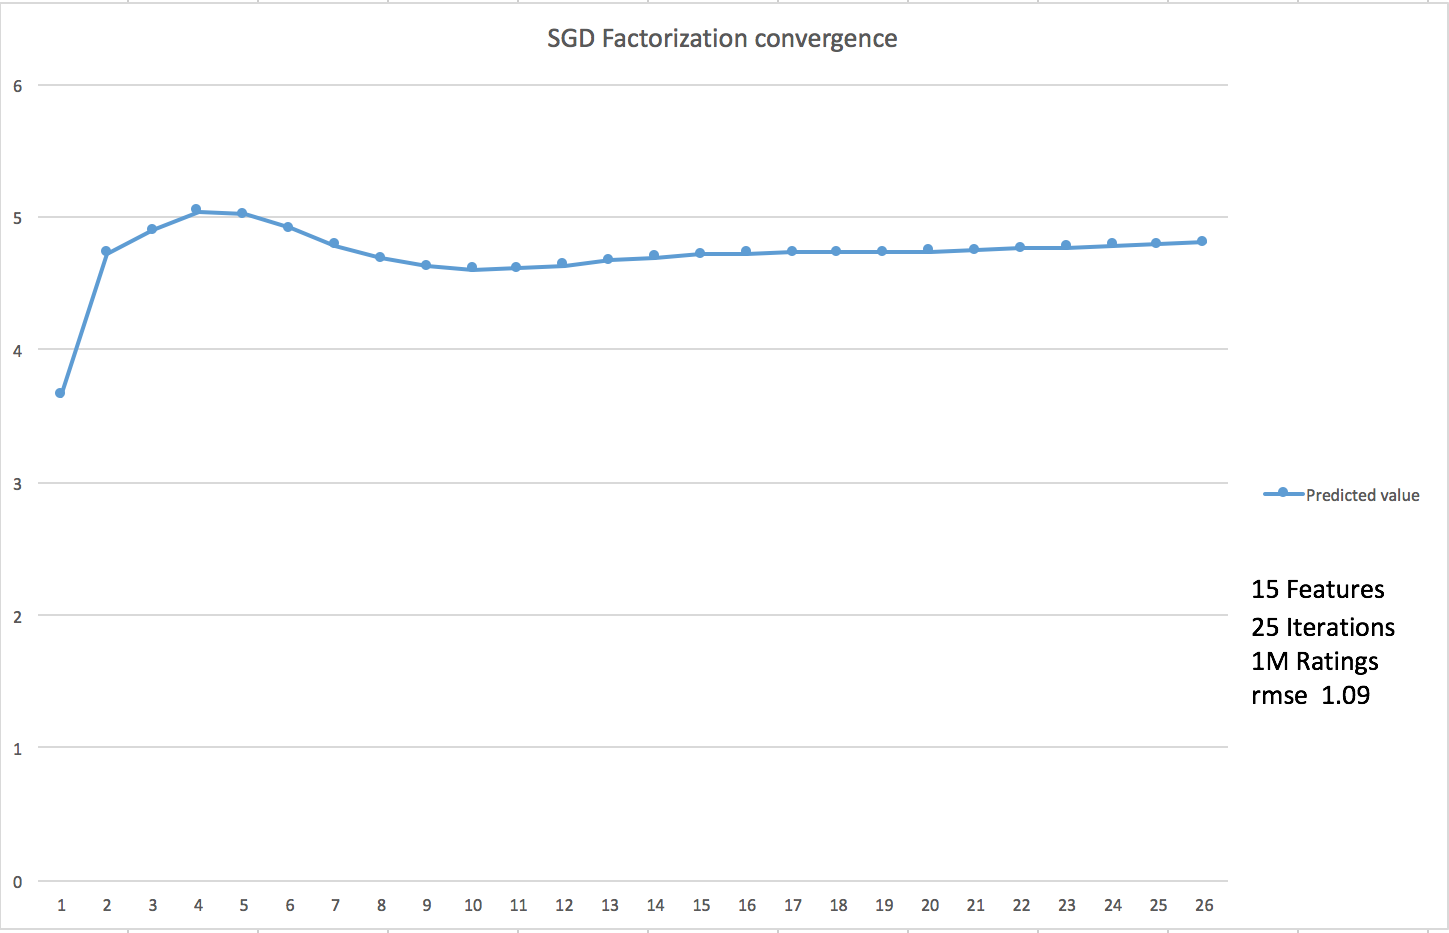
\includegraphics[scale=0.175]{chart.png}
\end{figure}


\subsection{Playing with the RMSE}
The most important factor and indicator of the whole algorithm is the \textit{root mean
square error}. The rmse indicates the "correctness" of the algorithm, in our case
a good value would be from 0.8 to 1.1 at maximum. The typical value for this dataset
is around 0.9[10].\\
Altough the algorithm was correct in our first batch of test the \textit{rmse} was
around 1.29, which is not the best value we could get. We tried to fine tune some
parameters, starting with the number of iterations and the number of features, the ones
we considered the most relevant in the algorithm. However we were wrong, the
error was not decreasing as expected but only of few decimal values.
The key to our high value was in the \textit{bias learning rate} or $\alpha$ in the pseudocode,
which was too high and was influencing too much the prediction. Using a value around 0.1 we decreased
the error of a factor of 32$\%$, with a resulting rmse = 0.9 on the test data and 0.88 on the training data,
which is a good result (see figure 3).
\begin{figure}
    \caption{Figure 3}
    \centering
    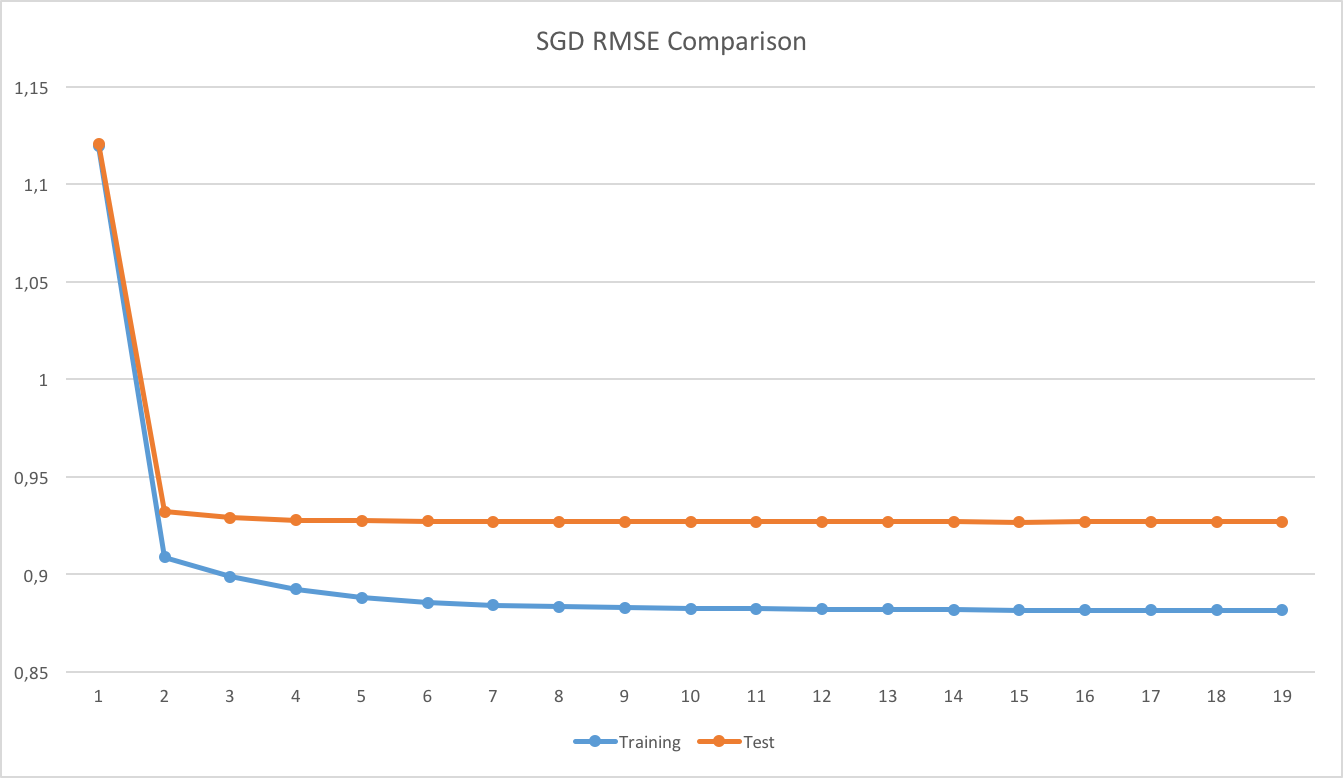
\includegraphics[scale=0.4]{sgdrmseserial.png}
\end{figure}


\subsection{The parallel version}
We analyzed the iterative version and in order to proceede in the parallelization
we had to find some indipendent parts in our code. We made the assumption
that all users may be processes indipendently even though the items will be shared.
We solved this problem using concurrency on the items allowing only one of the
parallel executions to have it. \\
We have sliced the execution assigning theoretically a thread to each slide
until the environment allows us to. In our case the maximum was 1500, but with
some fine tuning of the heap and stack parameters one can allocate around 100 thousands
of Java threads.[11]\\

\begin{algorithm}
    \caption{Matrix Factorization with parallel SGD}

    \begin{algorithmic}[1]
        \Require
            \Statex R is the user-item matrix,
            \Statex V and W are the factor vectors initialized with values from 0.0 to 1.0,
            \Statex $\alpha$ is the learning rate,
            \Statex $\lambda$ the magnitude reduction,
            \Statex K is the number of iterations
            \Statex F is the number of features
    \State shuffle(Ratings)
    \For{$i$ to  $K$ }
        \State run a thread for each user until the maximum number or the limit is reached
        \For{ each user $u$ }
            \For{ each item $i$ rated by $u$}
                \State lock(item $i$)
                \State $predictedRating = V[u] * W[i]^{t}$
                \State $error = R[u,i] - predictedRating$
                    \For{each feature $f \in F$}
                        \State $V[u,f] = V[u,f] + \alpha * (error * W[i,f] - \lambda * V[u,f])$
                        \State $W[i,f] = V[u,f] + \alpha * (error * V[i,f] - \lambda * W[u,f])$
                    \EndFor
                \State unlock(item $i$)
            \EndFor
        \EndFor
    \State wait for all threads to join
    \EndFor
    \end{algorithmic}
\end{algorithm}

Altough the parallel version of our algorithm needs some locking system
due to the concurrency on the items vector when reading and updating it
there is a theoretical approach to a more distributed version. The key
of this approach is to create a graph with all the interdepences between
users and items, where the edges are the correlations. If we have
more connected components, those will be fully independant from the others
because there will be no concurrency issue between items, therefore we
will be able to compute those on different machines and collect the results in the end.
The only problem is relative to the possible number of connected components which
is by nature of the problem very small, if not only one.




\section{Conclusions}
Research not always means finding the new disruptive innovation
or the coolest algorithm; most of the times you try
you make mistakes and most important of all you \textit{learn}.
We learned that very likely Scala is not the best programming language
for not parallel algorithms; maybe a C++ solution would have been faster as
expected. Maybe Stochastic Gradient Descent is not the best approach for matrix
factorization, which would explain why there is no Scala implementation yet
instead of the much more spreaded ALS.


%
% The following two commands are all you need in the
% initial runs of your .tex file to
% produce the bibliography for the citations in your paper.
\bibliographystyle{abbrv}
\bibliography{sigproc}  % sigproc.bib is the name of the Bibliography in this case
% You must have a proper ".bib" file
%  and remember to run:
% latex bibtex latex latex
% to resolve all references
%
% ACM needs 'a single self-contained file'!
%
%APPENDICES are optional
%\balancecolumns
\appendix
%Appendix A

\end{document}
